\begin{table}[t]
    \centering
    \caption{Estimated structural parameters}
    \begin{tabular}{ccc}
    \toprule
    & (1) & (2) \\
    & $b_2 = 0$ & $c_2 = 0$ \\
    \midrule
    $a_1$ & -0.182 & -0.182 \\
    $a_2$ & -0.150 & -0.150 \\
    $b_2$ && 0.040 \\
    $c_2$ & 0.826 \\
    \bottomrule
\end{tabular}

    \label{tab:results}
\end{table}

Table \ref{tab:results} shows the estimated values for $a_1$, $a_2$, $b_2$, and $c_2$ under both specifications. The estimated coefficients for $a_1$ and $a_2$ are virtually identical across both specifications, which justifies the assumption that we can zero out one of them and still measure the actual effect. The signs and magnitudes of our estimates are comparable to those found in other literature, including \textcite{blanchard2002empirical}.

One benefit to modeling an autoregressive process is the ability to observe the causal effect of a shock at time $t$ at later time periods. Because of the detrending process, the model has a 0 steady state for all three series. Starting from this steady state, we apply a government spending structural shock to the model that increases spending by 1\%. Then, the predictions at time $t$ are used for lags at time $t + 1$. Iterating this process gets the impulse response function (IRF), which shows the behavior of the model after the shock.

\begin{figure}[t!]
    \centering
    \caption{Estimated IRFs for a structural government spending shock}
    \begin{subfigure}{\textwidth}
        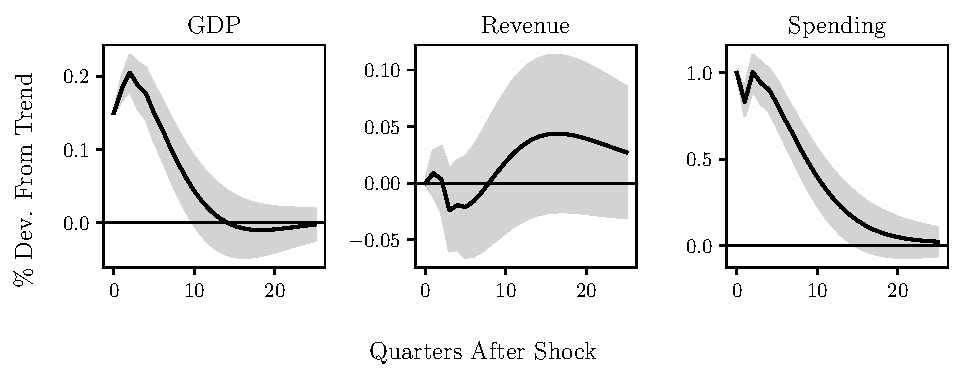
\includegraphics{figures/b20_irf.pdf}
        \caption{$b_2 = 0$}
    \end{subfigure}

    \begin{subfigure}{\textwidth}
        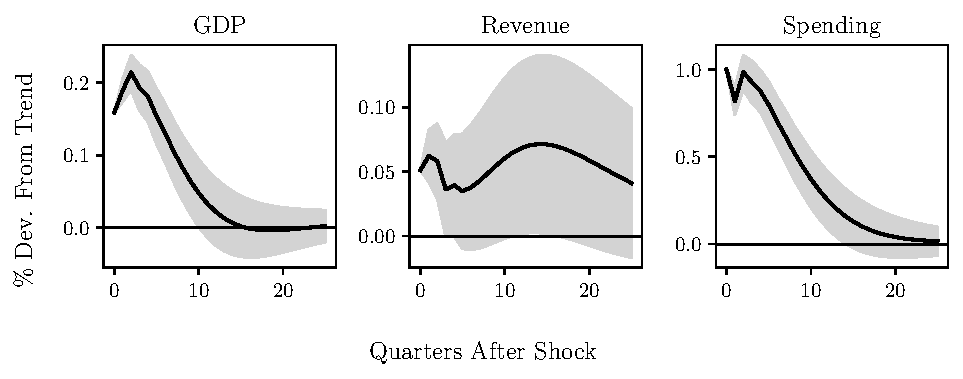
\includegraphics{figures/c20_irf.pdf}
        \caption{$c_2 = 0$}
    \end{subfigure}

    {\scriptsize \emph{Notes:} IRFs iterated for 25 periods.}
    \label{fig:irfs}
\end{figure}

Figure \ref{fig:irfs} shows the estimated IRFs for the two models. GDP and government spending follow the same paths across both specifications, again supporting the robustness of our results. Government revenues vary more between specifications but are both within the uncertainty interval of each other. The eigenvalues of the system have a magnitude less than one, so all three series eventually trend towards the steady state, demonstrating the short-run effects of business cycles \parencite{mitchell2024business}. Because government spending is shocked, it responds immediately. The largest increase in GDP happens slightly after the shock hits, meaning causal effect of the shock is delayed. The effect on government revenue happens much later, consistent with the idea that most government spending is deficit financed in the short run, then paid back well into the future \parencite{haley1941federal}.

Following \textcite{blanchard2002empirical}, the causal effect of the government spending shock is the maximum effect along the IRF. An alternative approach would examine the integral of the whole curve, but since GDP is a flow, not stock, variable, we view the single period increase as more important \parencite{deleidi2023government}. The causal effect is adjusted by the average GDP to government spending ratio to get the dollar effect on GDP of a dollar increase in government spending.

The $b_2 = 0$ model predicts a \$1 structural shock to government spending would increase GDP by \$0.990 with a standard error of \$0.115 and the $c_2 = 0$ model predicts the shock would increase GDP by \$1.035 with a standard error of \$0.115. Since GDP includes government spending, both estimates suggest the GDP effect of the spending shock is entirely the spending increase from the shock. Therefore, we find no evidence of either crowding out or multiplier effects.
